\chapter{Results and Discussion}
\label{cha:results}
\section{Numerical Tests in an 2D Toy Potential}
\label{sec:2D}
As a simple test to check all ABM methods a single particle in the two-dimensional potential $U_2$ (eq.~\ref{eq:U2}) is considered.
By performing a simple 2D to 2D mapping in the absence of any dimensionality reduction, the analytical PMF and free energy difference is given by
\begin{equation}
  \begin{split}
    A(x,y)&=U_2(x,y) \\
    \Delta A_{A\to B} &= 0
  \end{split}
\end{equation}
The convergence of numerical PMFs and free energy differences to the analytical result with different adaptive biasing schemes (MtD, WTM, ABF, eABF and WTM-eABF) is computed over the course of 5~ns trajectories.
Note that all adaptive biasing methods depend on a different set of parameters.
Their convergence can therefore only be compared qualitatively.
A detailed analysis of the impact of the choice of parameters will be given in the following section.
Parameters applied in this section and resulting PMFs after 1, 3 and 5~ns are given in the Appendix.
In Fig.~\ref{fig:conv 2D} the convergence of the PMF and corresponding estimate for the free energy difference over time is given.
Fig.~\ref{fig:error 2D} shows remaining absolute local errors at the end of all simulations.

In an unbiased simulation the system stays trapped in one metastable state.
This is a example of quasi-nonergodic behavior, where simple time averages of MD trajectories do not converge to the correct ensemble average.
Because only a small region of CV space is explored the free energy difference $\Delta A_{A\to B}$ is highly overestimated.

All adaptive biasing methods reduce the metastability significantly and enable uniform sampling of both states.
In MtD/WTM simulations the PMF is given by a superposition of Gaussian hills, which are deposited linearly over time and fill both minima consecutively.
For this particular set of parameters no full convergence is reached in 5~ns.
Regions with high free energy at the margins remain unexplored due to incomplete filling of the PMF with Gaussians and the obtained PMFs deviate from the analytic result by about 20~\%.
However, using WTM this is intentional as the fraction of the PMF that is compensated in the simulation is chosen with the effective temperature $\Delta T$.
The height of Gaussians is reduced over time, which results in significantly smaller fluctuations and absolute errors of the PMF in large parts of the PMF than with MtD.
After 4~ns the free energy difference $\Delta A_{A\to B}$ obtained from WTM therefore converges safely towards 0~kJ/mol.
\begin{figure}[H]
   \centering
   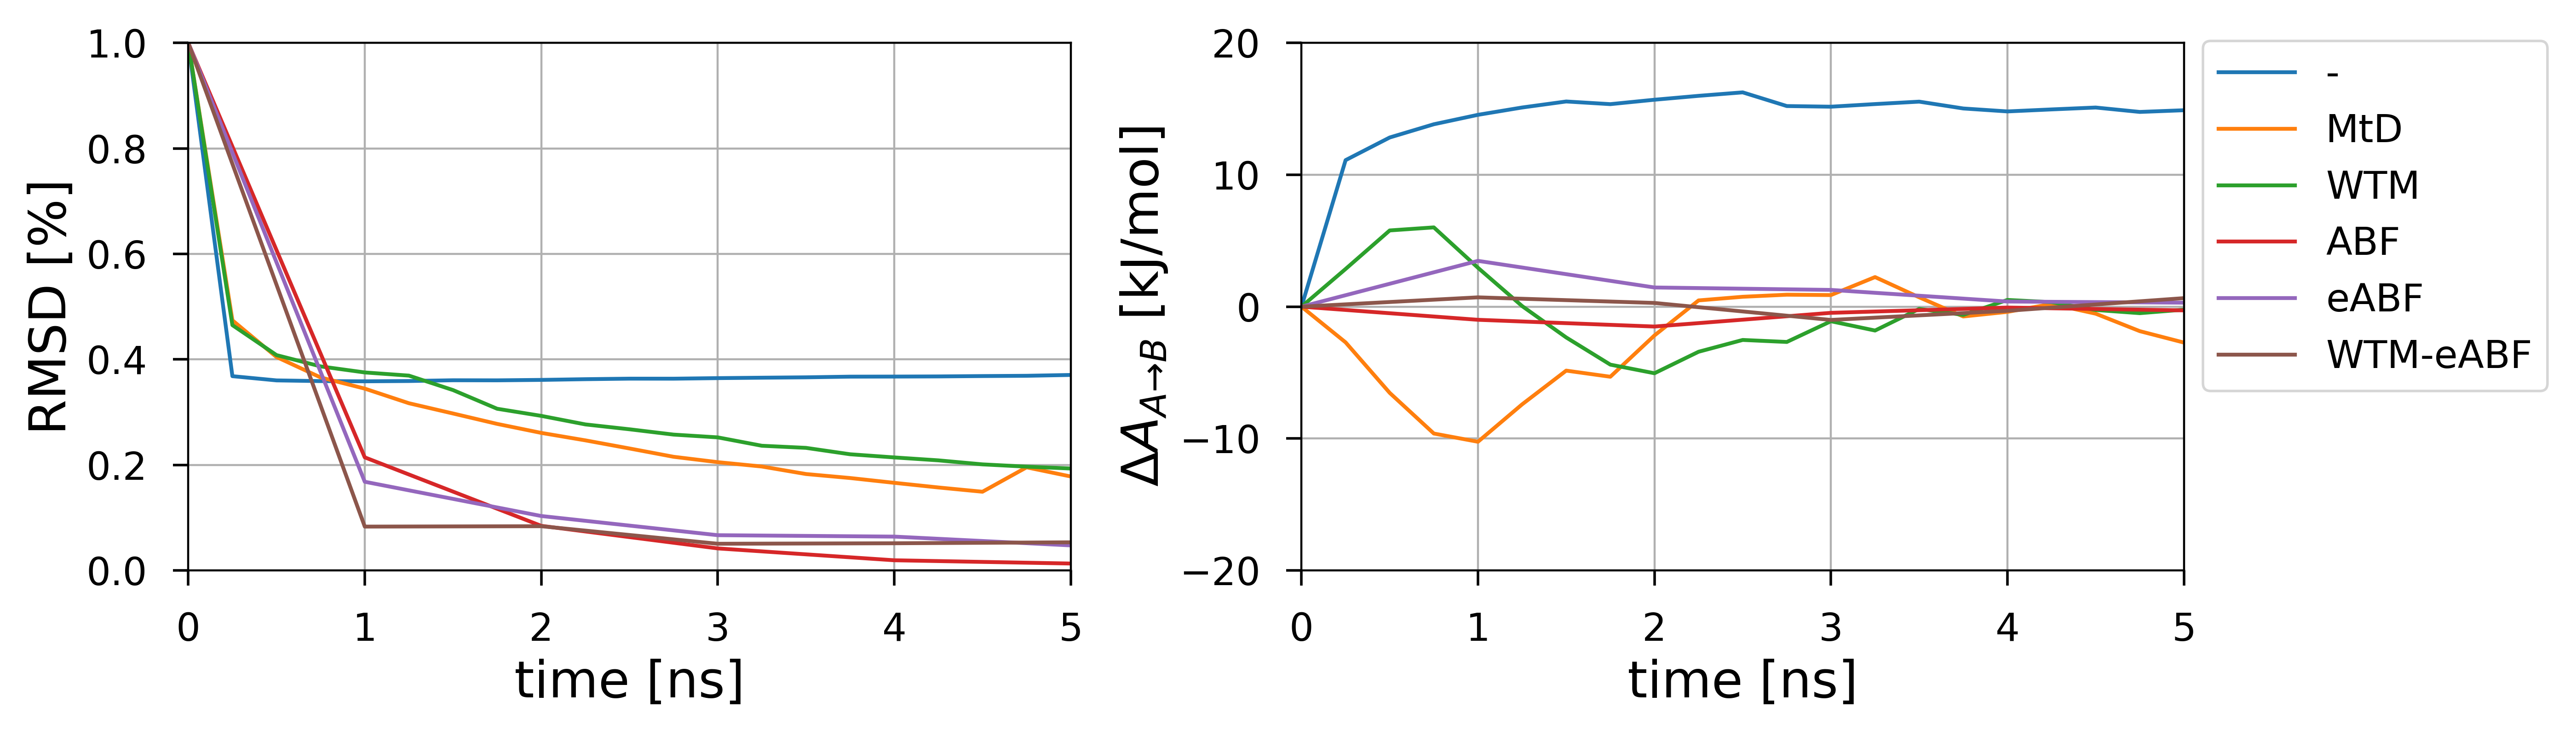
\includegraphics[width=0.99\textwidth]{bilder/test_2D/conv}
   \caption{Convergence of free energy calculations with different adaptive biasing methods for a 2D to 2D mapping of toy potential $U_2$. On the right the RMSD between the analytical and numerical PMF is given over the course of 5~ns trajectories. On the right the development of free energy differences $\Delta A_{A\to B}$ given by eq.~\ref{eq:free energy diff} is shown. Both metastable states are separated by the line $0.25x+y$. Therefore $A$ includes all states $x>-4y$ and $B$ all states $x<-4y$, respectively.}
 \label{fig:conv 2D}%
\end{figure}
\begin{figure}[H]
  \centering
  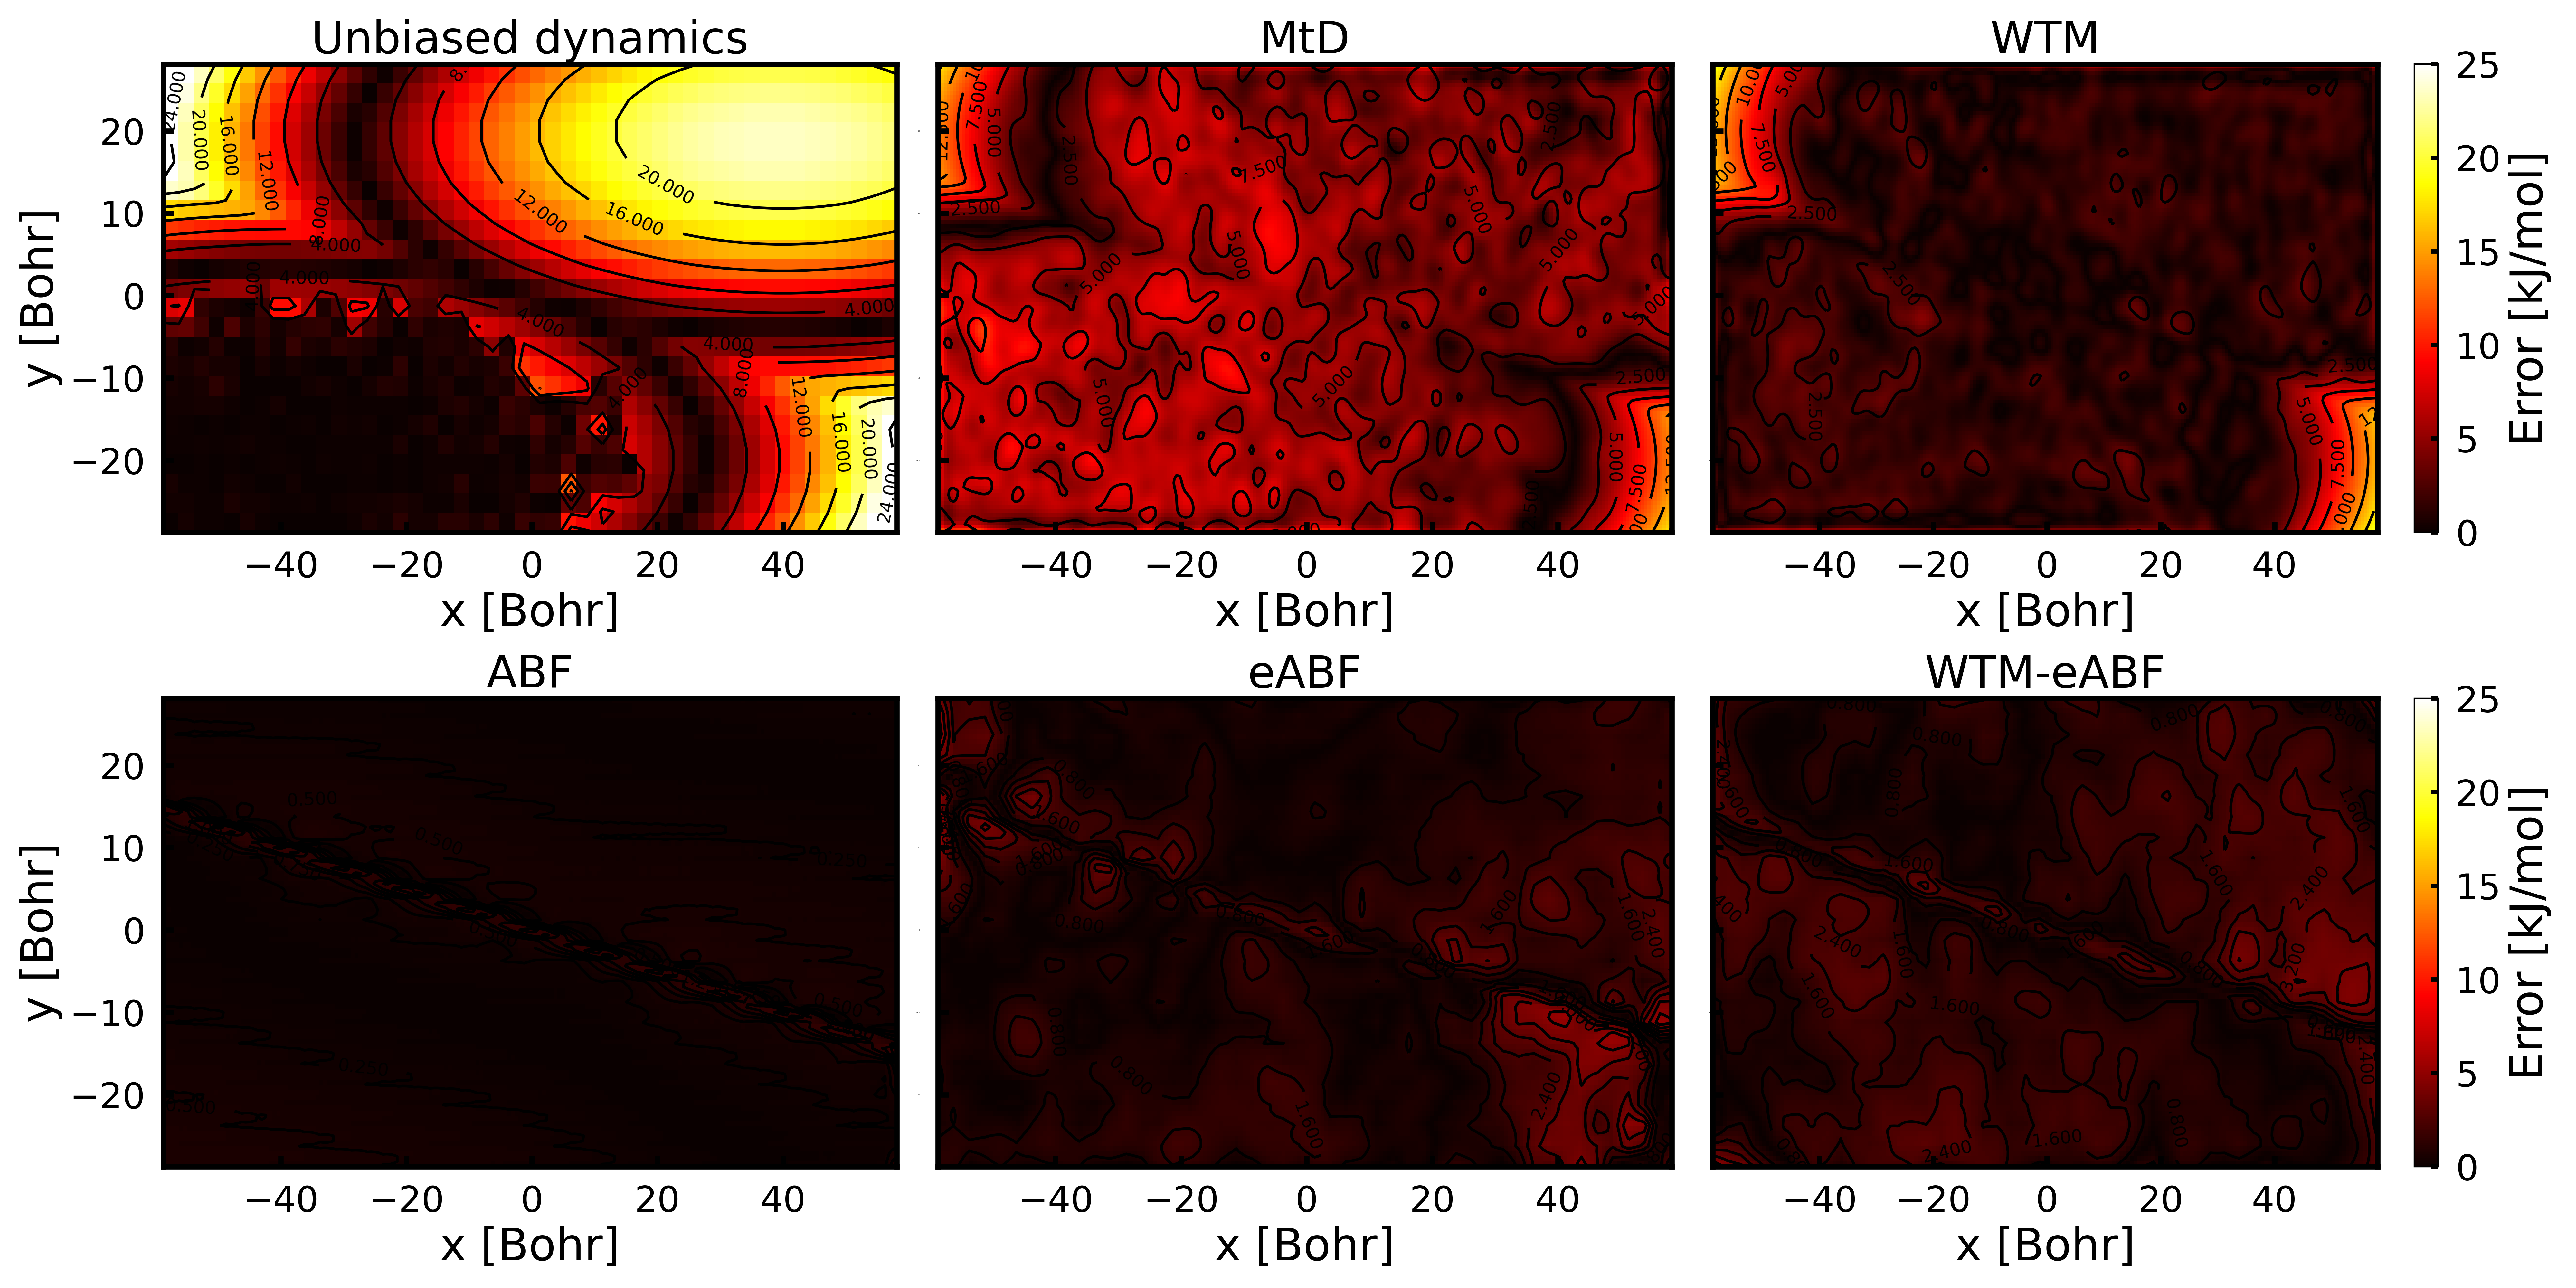
\includegraphics[width=0.99\textwidth]{bilder/test_2D/error_5ns}
  \caption{Heat maps of the absolute difference between the analytic and numerical PMFs. Numerical PMFs are obtained from 5~ns MD trajectories at 300~K.}
\label{fig:error 2D}%
\end{figure}
With ABF after 3~ns the potential is mapped almost perfectly with maximum local errors below 1~kJ/mol. Also the RMSD of the PMF and free energy difference $\Delta A_{A\to B}$ converges rigorously to the analytic results.
For this particular example ABF force samples are simply given by the gradient of the analytical potential.
The variance of force samples, which is only introduced by the finite bin width, is therefore small and convergence of the ABF force in individual bins is reached almost instantly.
Even faster exploration of the PMF is only hindered by the ramp function, which is not strictly necessary for this toy example, but still applied to provide a more realistic test case for real chemical applications.
PMFs are obtained by thermodynamic integration of ABF forces with the FEM method, as shown in Fig.~\ref{fig:ti}.
\begin{figure}[H]
  \centering
  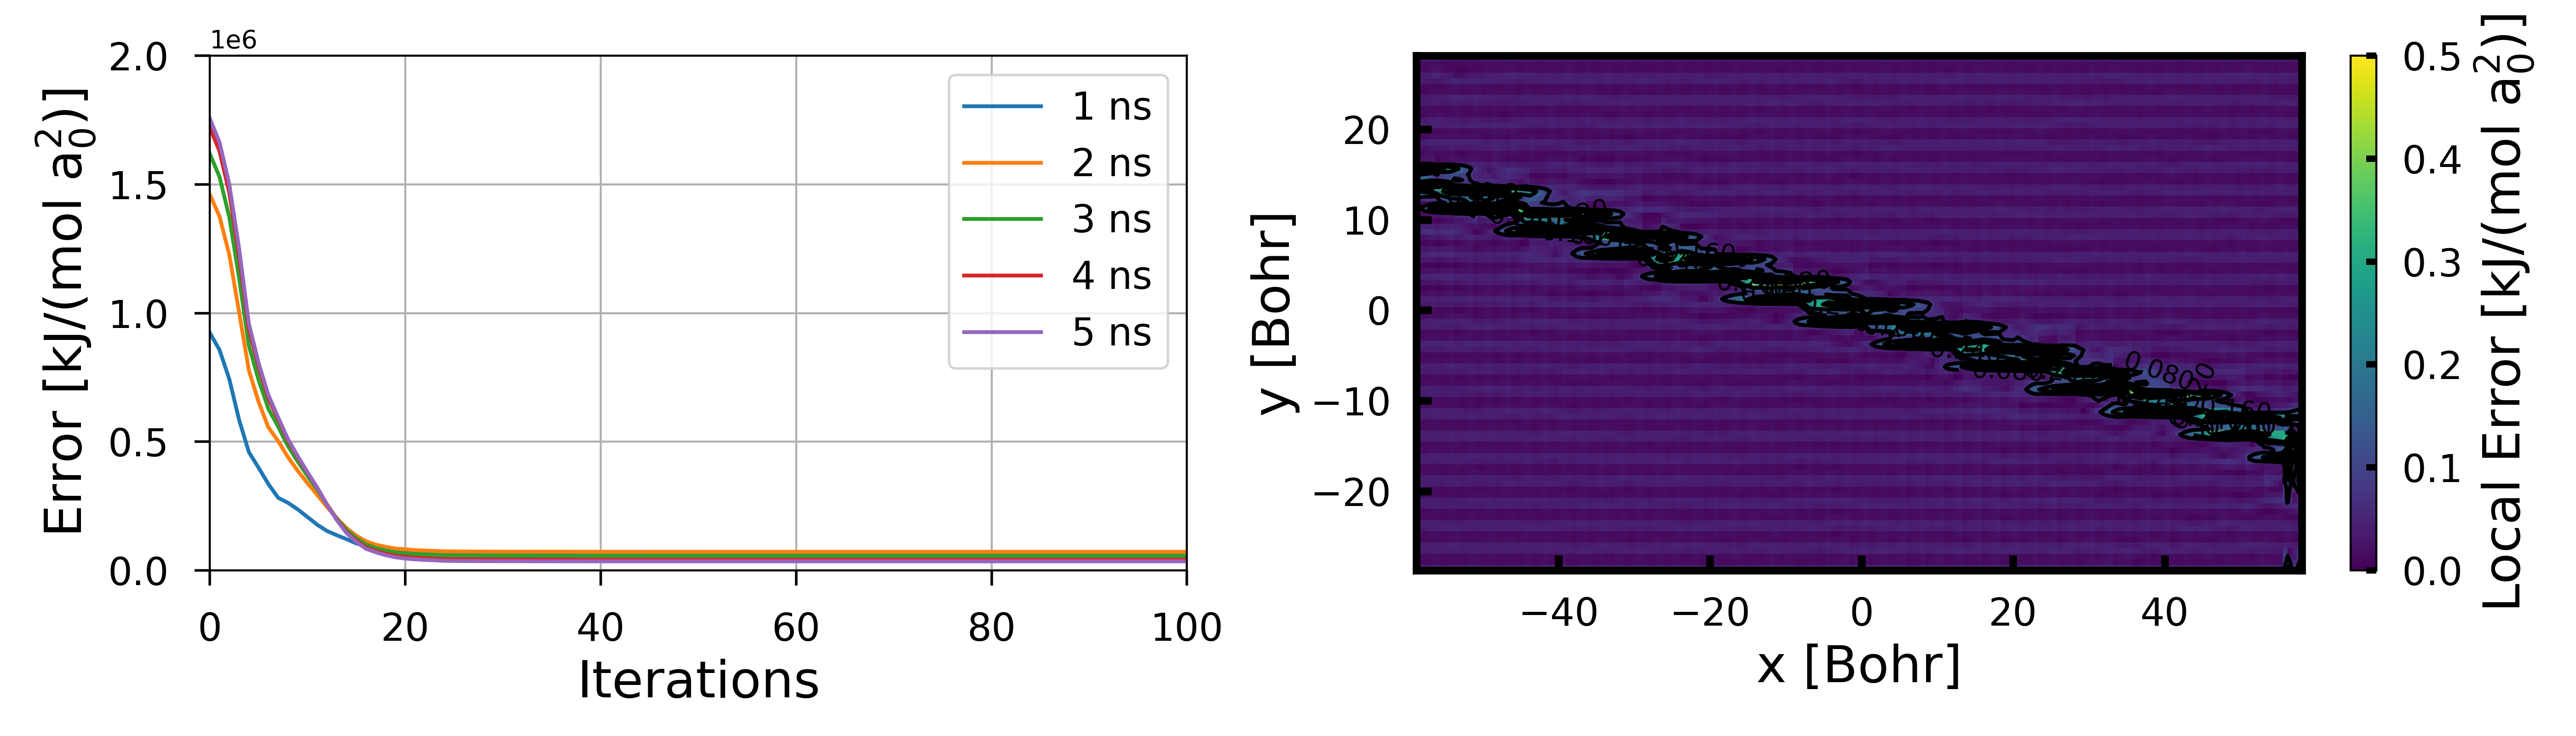
\includegraphics[width=0.99\textwidth]{bilder/test_2D/ti}
  \caption{On the left the convergence of the thermodynamic integration of ABF forces with the FEM method in a BFGS minimization is given for different time steps. On the right the mean local difference of optimized B-splines to the mean forces is shown.}
\label{fig:ti}%
\end{figure}
Convergence of the FEM method is reached reliably in 100 iterations by minimization of eq.~\ref{eq:RMSD} with the BFGS algorithm.
At the transition barrier, where the thermodynamic force changes rapidly, this introduces small errors to the PMF, which can be reduced with a smaller bin width and more B-spline functions.

Both eABF and WTM-eABF preserve the rigorous convergence behavior of ABF.
By estimating the thermodynamic force over the extended-system, the variance of obtained force samples depends on the harmonic force constant of the coupling of the fictitious to the physical particle.
For this toy example this introduces some noise to the mean force, where it would reduce said noise in real chemical applications.\autocite{lesage2017smoothed}
The PMF therefore shows small fluctuations of up to 2~kJ/mol for both methods and convergence to the true PMF is reached with a final RMSD of about 2~\%.
However, quite surprisingly convergence of the mean force with eABF is as fast as with ABF and WTM-eABF gives an additional speed up.
With WTM-eABF the estimate for the free energy difference stays close to 0~kJ/mol over the course of the hole simulation.
This indicates that the hole PMF is explored uniformly from the beginning and the system is never trapped in one state.

In this section the favorable convergence behavior of ABF, eABF and WTM-eABF was demonstrated.
In the following sections this methods will be discussed in further detail for a real chemical system with special focus on the influence of input parameters on the simulations.

\newpage
\section{Benchmark Calculations for the Torsion of Cl-F-Ethane}
\label{sec:test}
The following section will give a detailed discussion on the effect of different parameters on the time convergence of adaptive biasing force methods (ABF, eABF and WTM-eABF).
As test system the transition of the dihedral angle between the Cl- and F-group in Cl-F-Ethane from the gauge$^+$ ($60^\circ$) to the gauge$^-$ ($-60^\circ$) structure on the PBEh-3c/dev2-msvp level of theory in vacuum will be considered.

Figure~\ref{fig:ABF benchmark} shows PMFs obtained from ABF calculations with different values of $N_{full}$ in 50~ps trajectories and the time convergence of free energy differences and RMSD of the PMF in reference to the final ABF ($N_{full}=100$) result.
After roughly 30~ps all three PMFs converge to the same result within 1.0~\% deviation.
For high values of $N_{full}$ it takes longer to fill the ramp functions.
This delays diffusion to the second minimum and uniform sampling of the reaction coordinate.
Small values of $N_{full}$ are associated with a certain risk to drive the system away from thermal equilibrium at the beginning of the simulation.
As instantaneous force samples depend on all molecular coordinates, the variance of fluctuations in estimates of the mean force grows with the system size.
More specifically this fluctuations are dominated by high frequency terms due to bonded interactions\autocite{lesage2017smoothed}, which also leads to a dependence of the variance in ABF force samples on the amount of equillibration prior to the simulation.\autocite{blondel2004ensemble}
In this example the result are large fluctuations of $\Delta A$ over the course of the simulation.
Overall $N_{full}=100$ is found to result in a good compromise between fast and stable convergence of the PMF and free energy difference.
\begin{figure}[H]
    \centering
    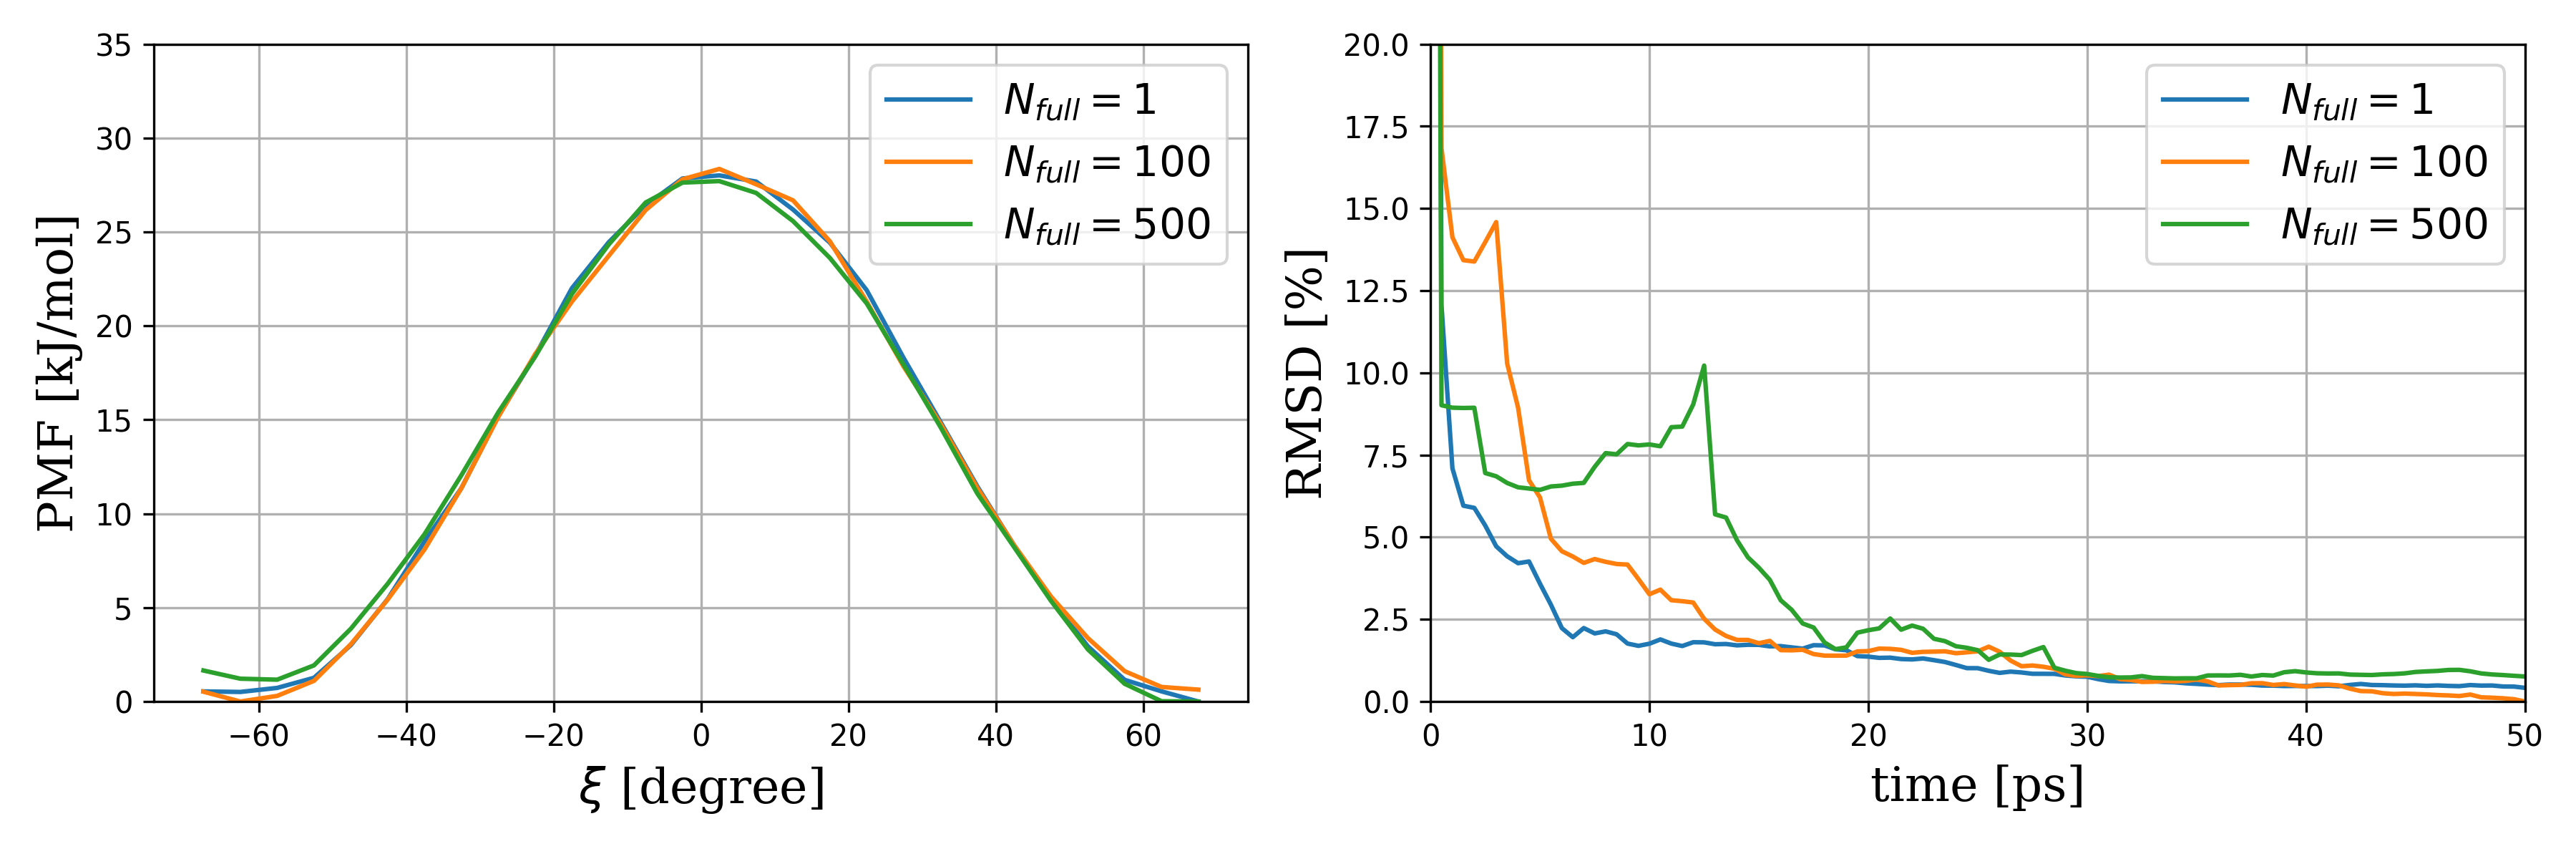
\includegraphics[width=0.99\textwidth]{bilder/benchmark/ABF_benchmark_nfull}
    \caption{ABF benchmark}
    \label{fig:ABF benchmark}
\end{figure}
In eABF calculations mean square fluctuations $\sigma_F$ of force samples only depend on the spring force between the CV and extended variable and are inversely proportional to the thermal width $\sigma_\lambda$.
\begin{equation}
    \sigma_F^2 \propto \frac{k_\lambda}{\beta} = \frac{1}{\beta\sigma_\lambda}
\end{equation}
The choice of $\sigma_\lambda$ is therefore a trade-off between enhanced sampling of the CV by tight coupling to $\lambda$ and reduced fluctuations of the extended force.\autocite{lesage2017smoothed}
Figure~\ref{fig:conf eABF} shows both limiting cases.
With a small thermal width of $1^\circ$ convergence is hindered by high fluctuations of the mean force.
On the other hand for loose coupling to the fictitious particle ($N_{full}=20^\circ$) $\lambda$ is sampled uniformly, but the physical CV stays trapped in one metastable state.
The mass of the extended variable has much less influence on the resulting PMF.
If the mass of the fictitious particle is much smaller than that of the CV, it is more difficult to pull the CV over the TS and convergence is slowed down.
However, no consistent influence of $m_\lambda$ on the obtained PMF is observed.
Relatively large scattering in the estimates of $\Delta A$ from $-2$~kJ/mol to $2$~kJ/mol indicate that no full convergence is reached 50~ps.
To calculate $\Delta A$ the probability of finding the system in the gauge$^-$ or gauge$^+$ state is obtained by integrating the corresponding probability densities, which are separated at the maximum of the PMF.
Therefore, small fluctuations of the PMF at the TS can lead to large shifts of $\Delta A$, because the maximum of the PMF switches to different bins.
\begin{figure}[H]
  \centering
    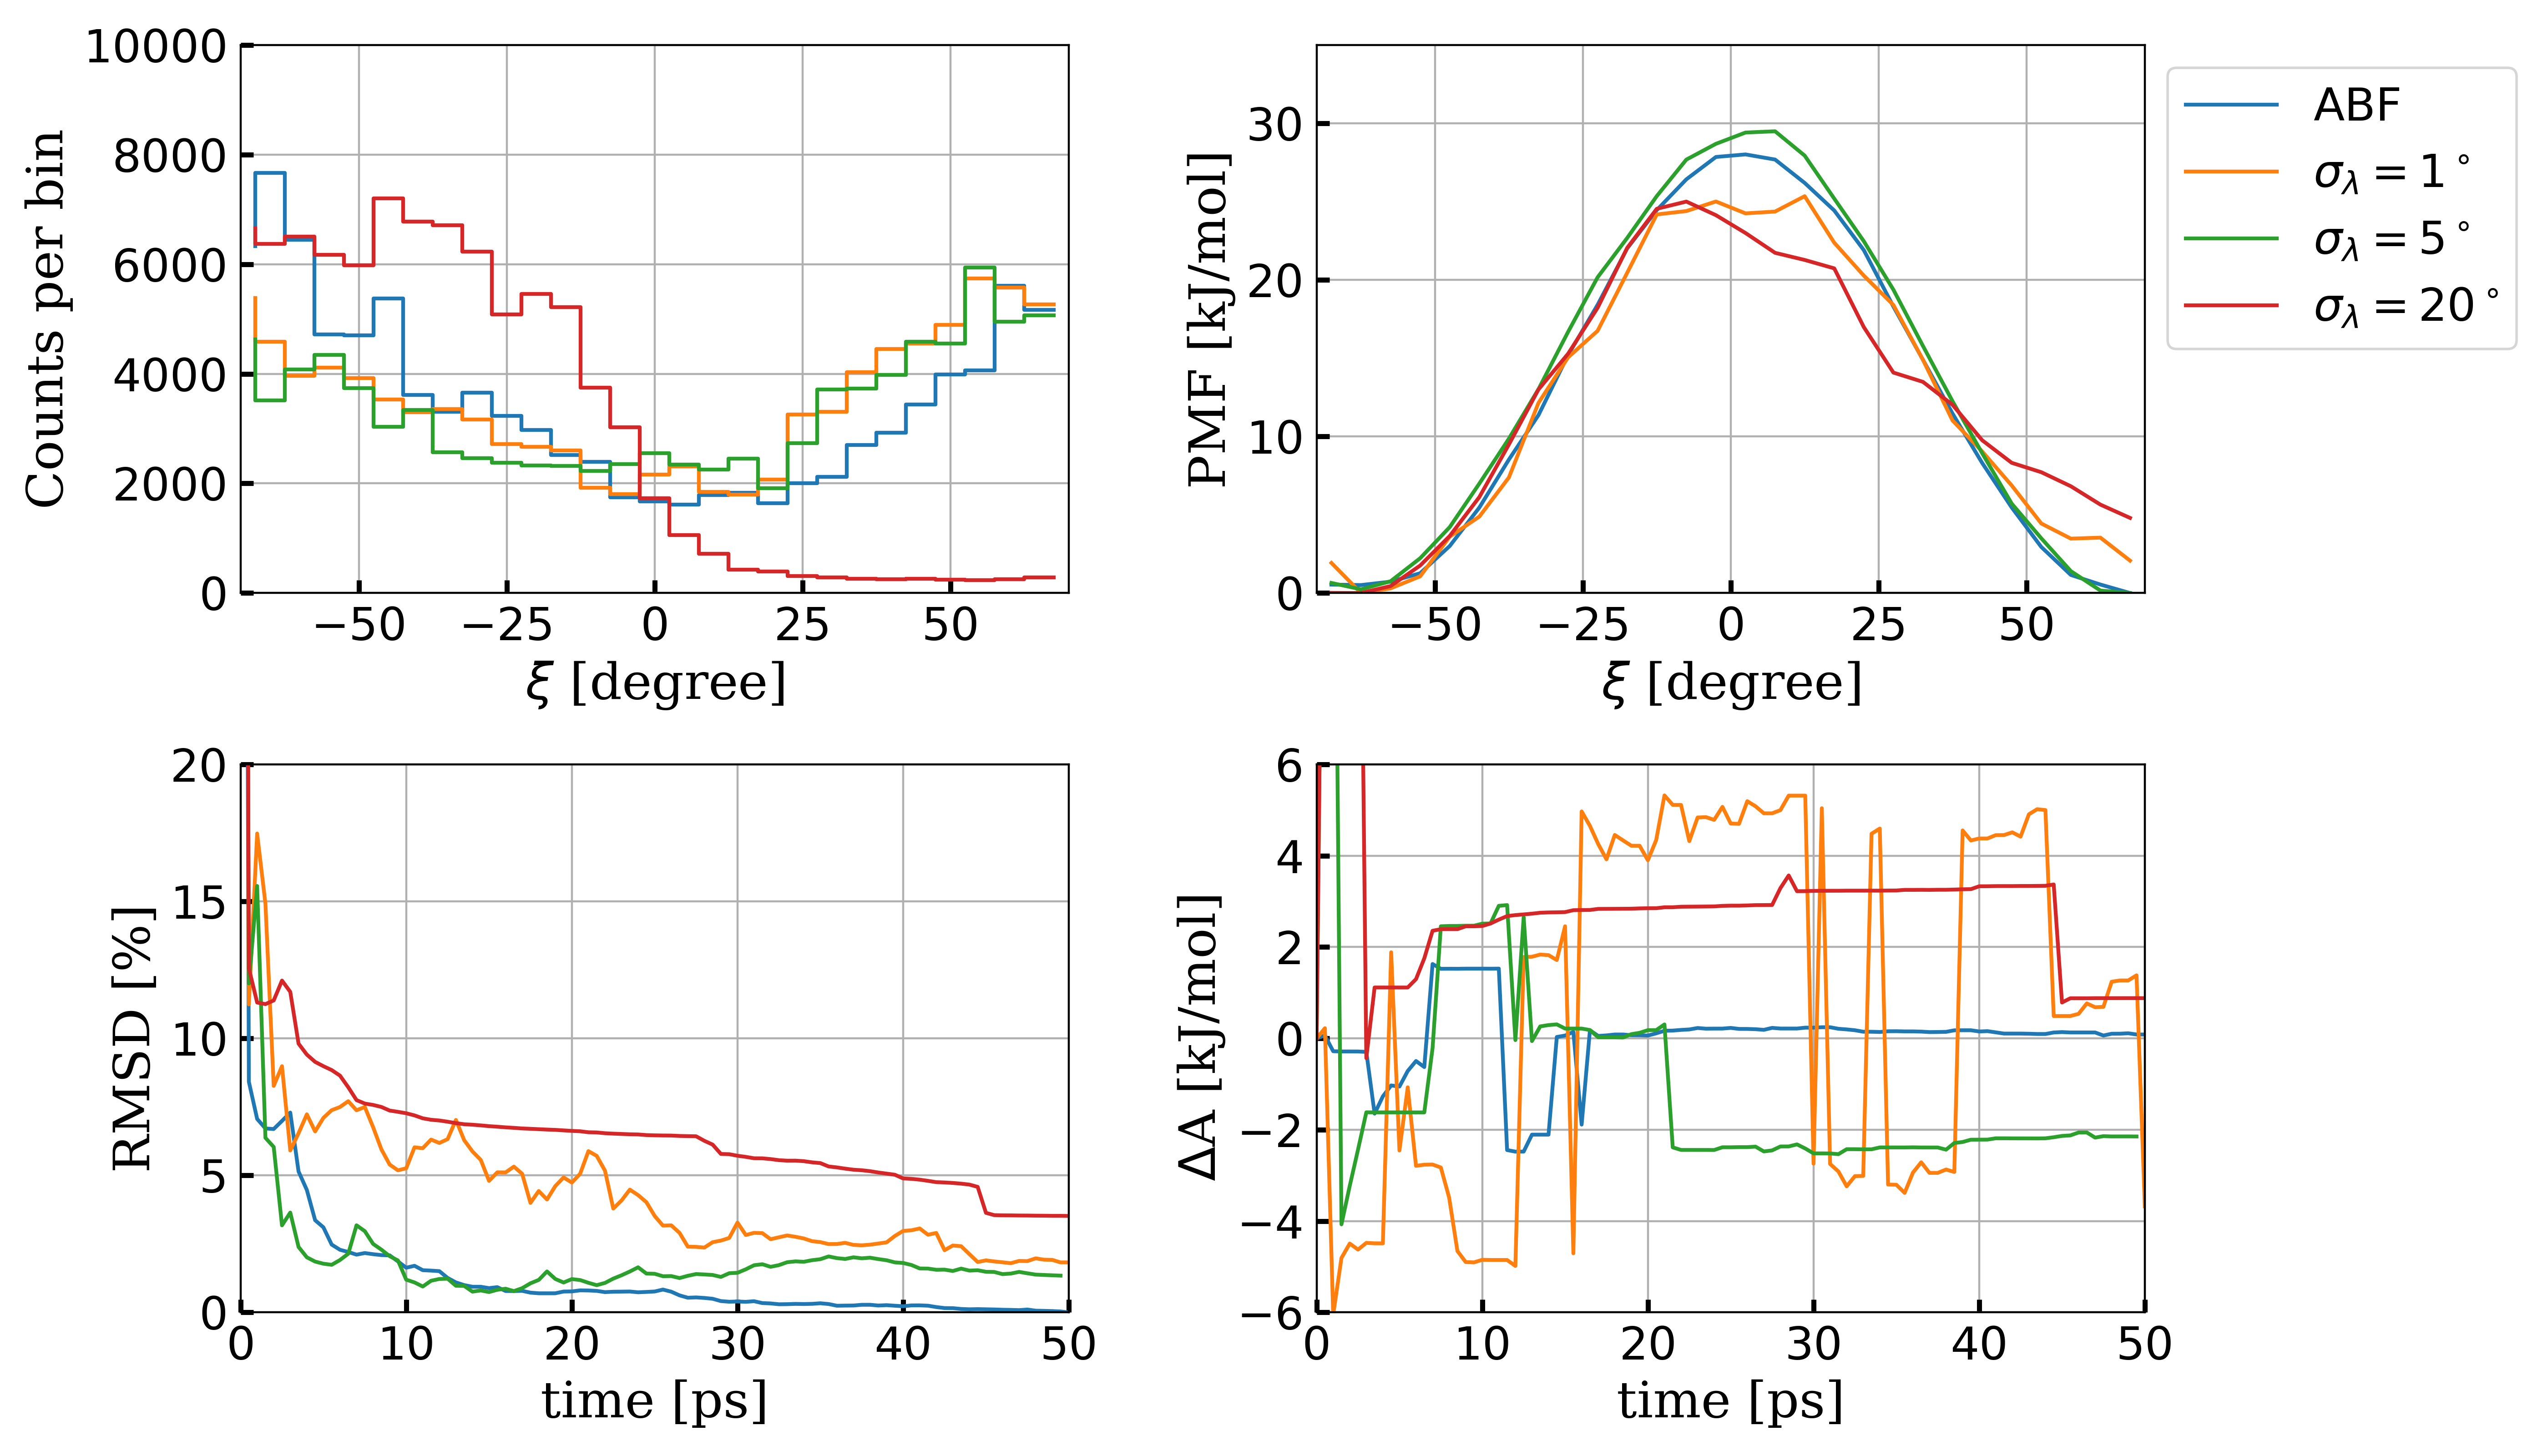
\includegraphics[width=0.99\textwidth]{bilder/benchmark/eABF_benchmark_sigma}
    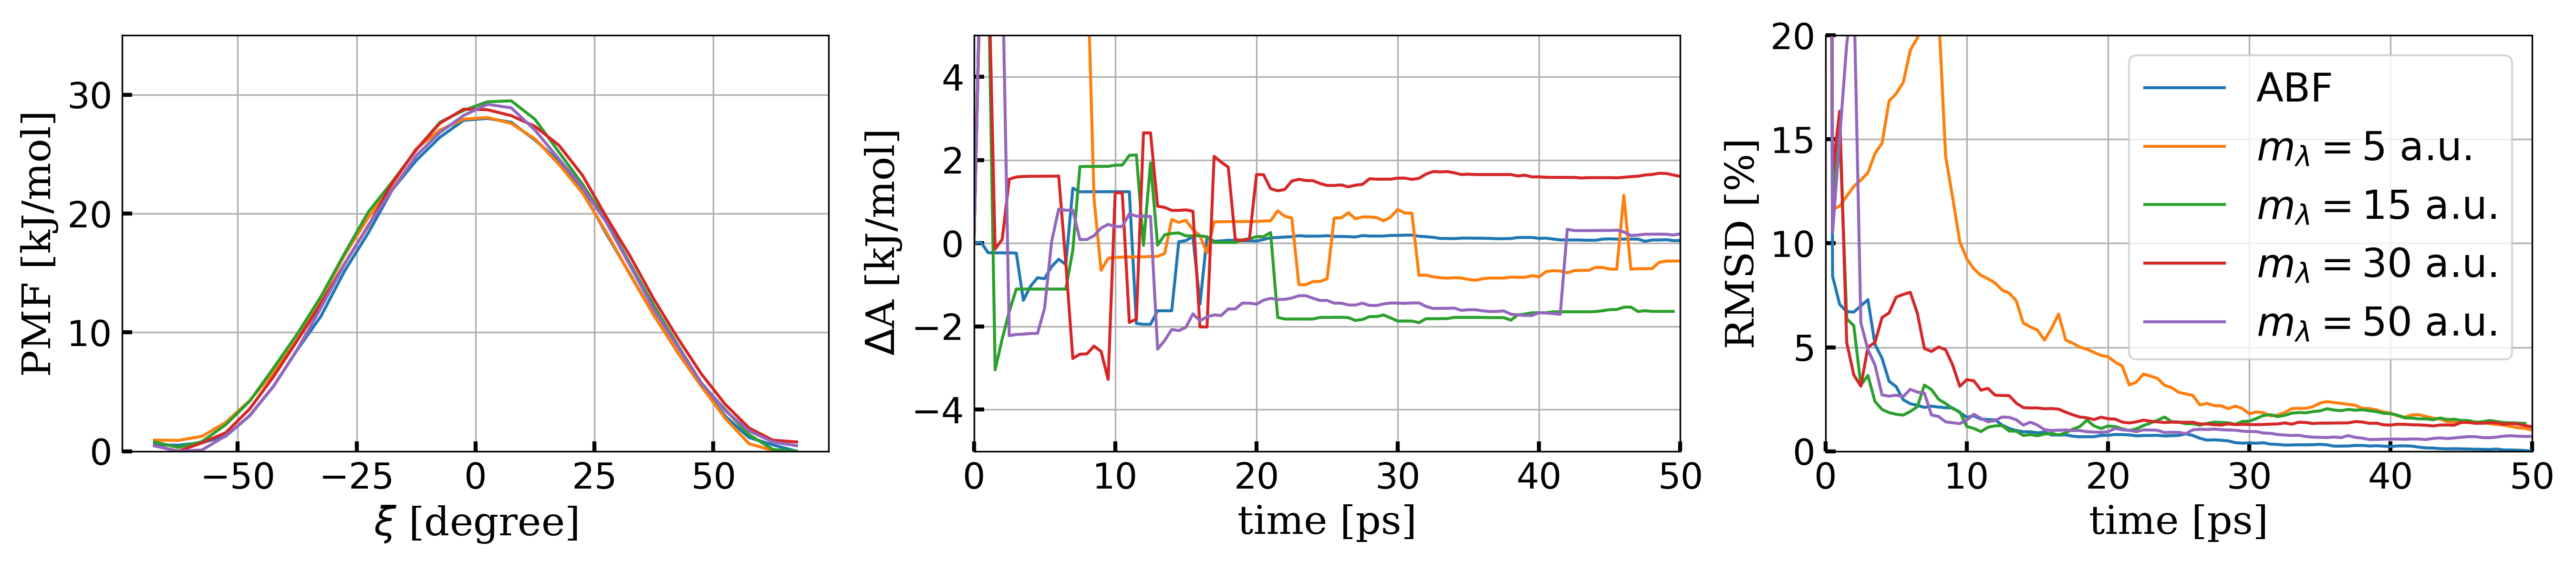
\includegraphics[width=0.99\textwidth]{bilder/benchmark/eABF_benchmark_mass}
   \caption{Convergence of eABF/CZAR with $m_\lambda=15$~a.u. and $N_{full}=100$.}
   \label{fig:conf eABF}
\end{figure}
Figure~\ref{fig:traj ABF} shows trajectories of simulations with ABF, eABF and WTM-eABF.
In WTM-eABF the number of transitions between both states is double as high is in a eABF normal ABF simulation with the same parameters of the extended-system.
This enables not only consistently faster convergence of the PMF, but also a more accurate result at the important TS region, as shown in Figure~\ref{fig:conf meABF}.
The fluctuations in the estimate of $\Delta A$ are therefore much smaller.
The WTM potential only enhances sampling by pushing the system to high free energy regions.
It has no significant impact on the resulting PMF, which is obtained from CZAR, as long the canonical ensemble is sampled.
WTM-eABF is therefore vary robust to the choice of WTM parameters like the Gaussian height $W$ and variance $\sigma_G$.
The influence of the eABF $m_\lamba$ and $\N_{full}$ is also even less severe, as both only impact enahanced sampling as well, which is always improved by the repulsive WTM potential.
\begin{figure}[H]
  \centering
    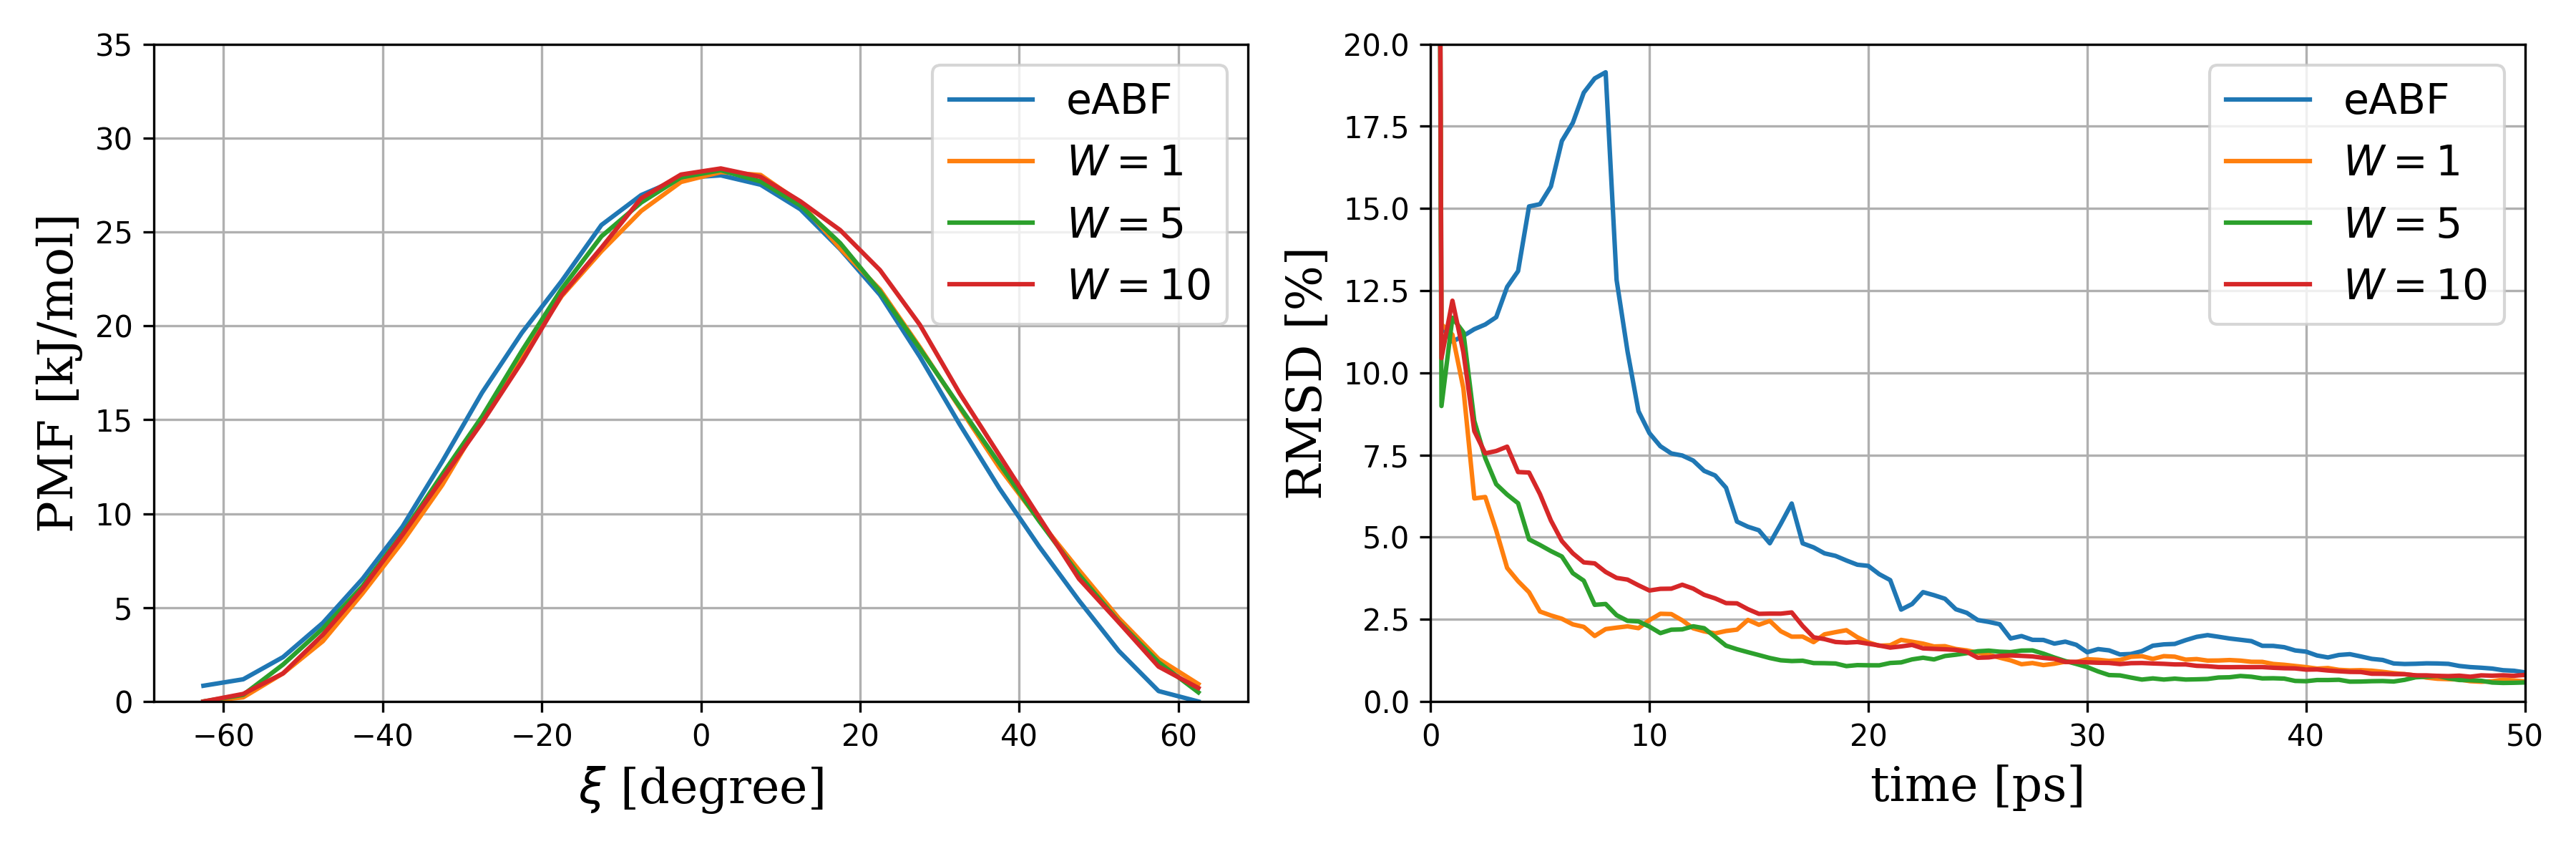
\includegraphics[width=0.99\textwidth]{bilder/benchmark/meta_eABF_benchmark_height}
    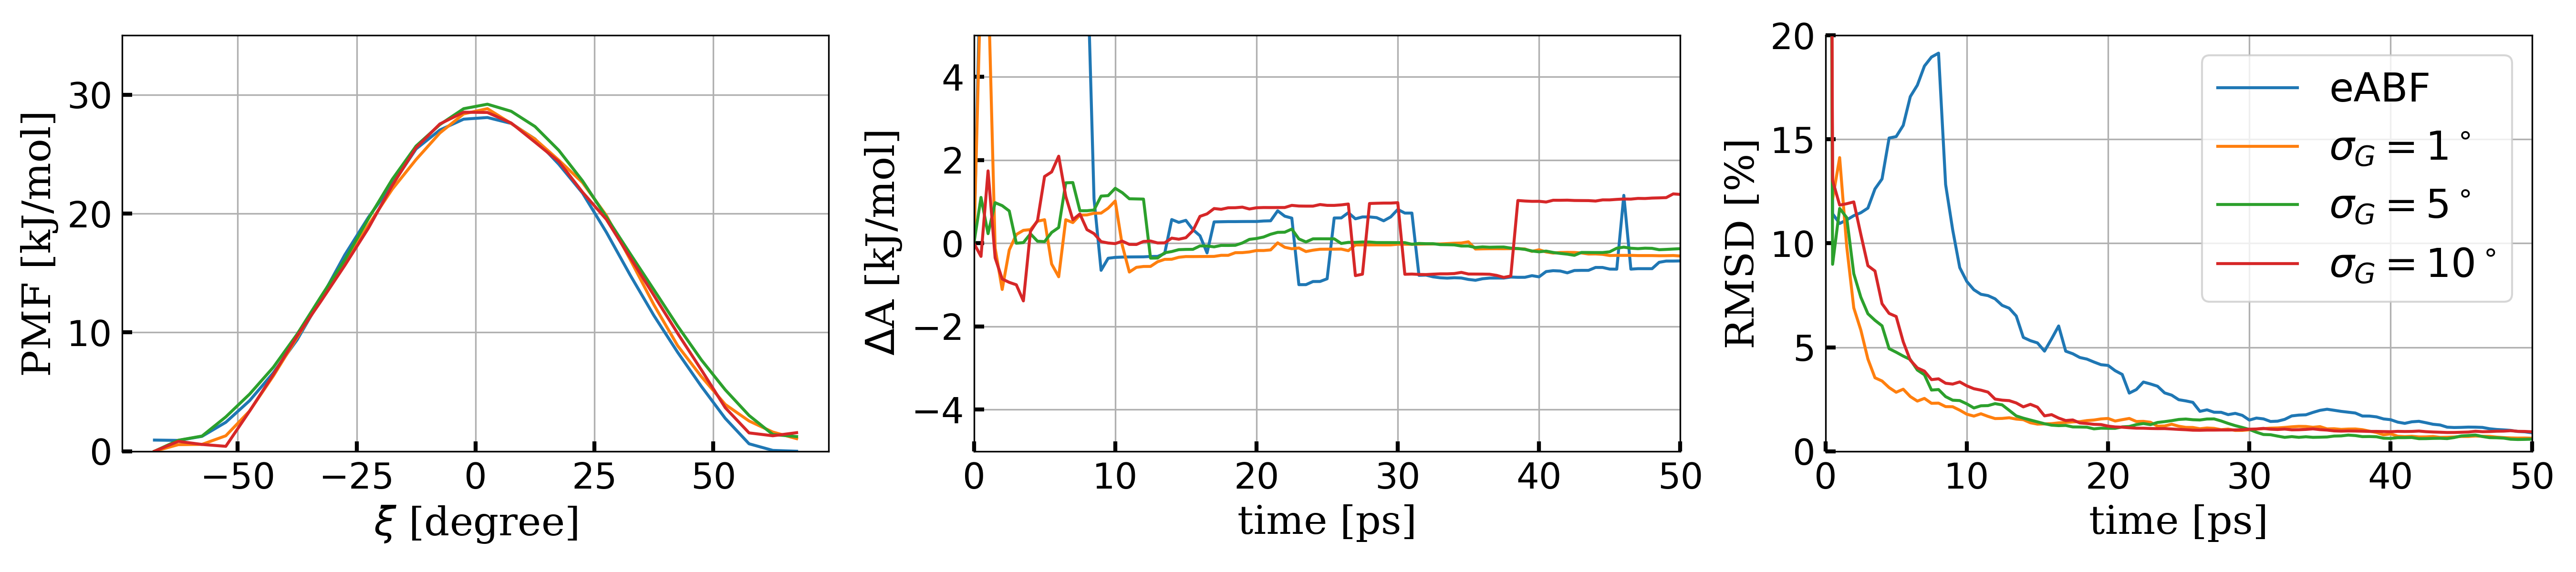
\includegraphics[width=0.99\textwidth]{bilder/benchmark/meta_eABF_benchmark_var}
   \caption{Convergence of WTM-eABF with $m_\lambda=5$~a.u., $\sigma_\lambda=5$, $\sigma_G=5$, $\tau_G=10$~fs, $\Delta T=2000$~K and $N_{full}=100$.}
   \label{fig:conf meABF}
\end{figure}
\begin{figure}[H]
     \centering
     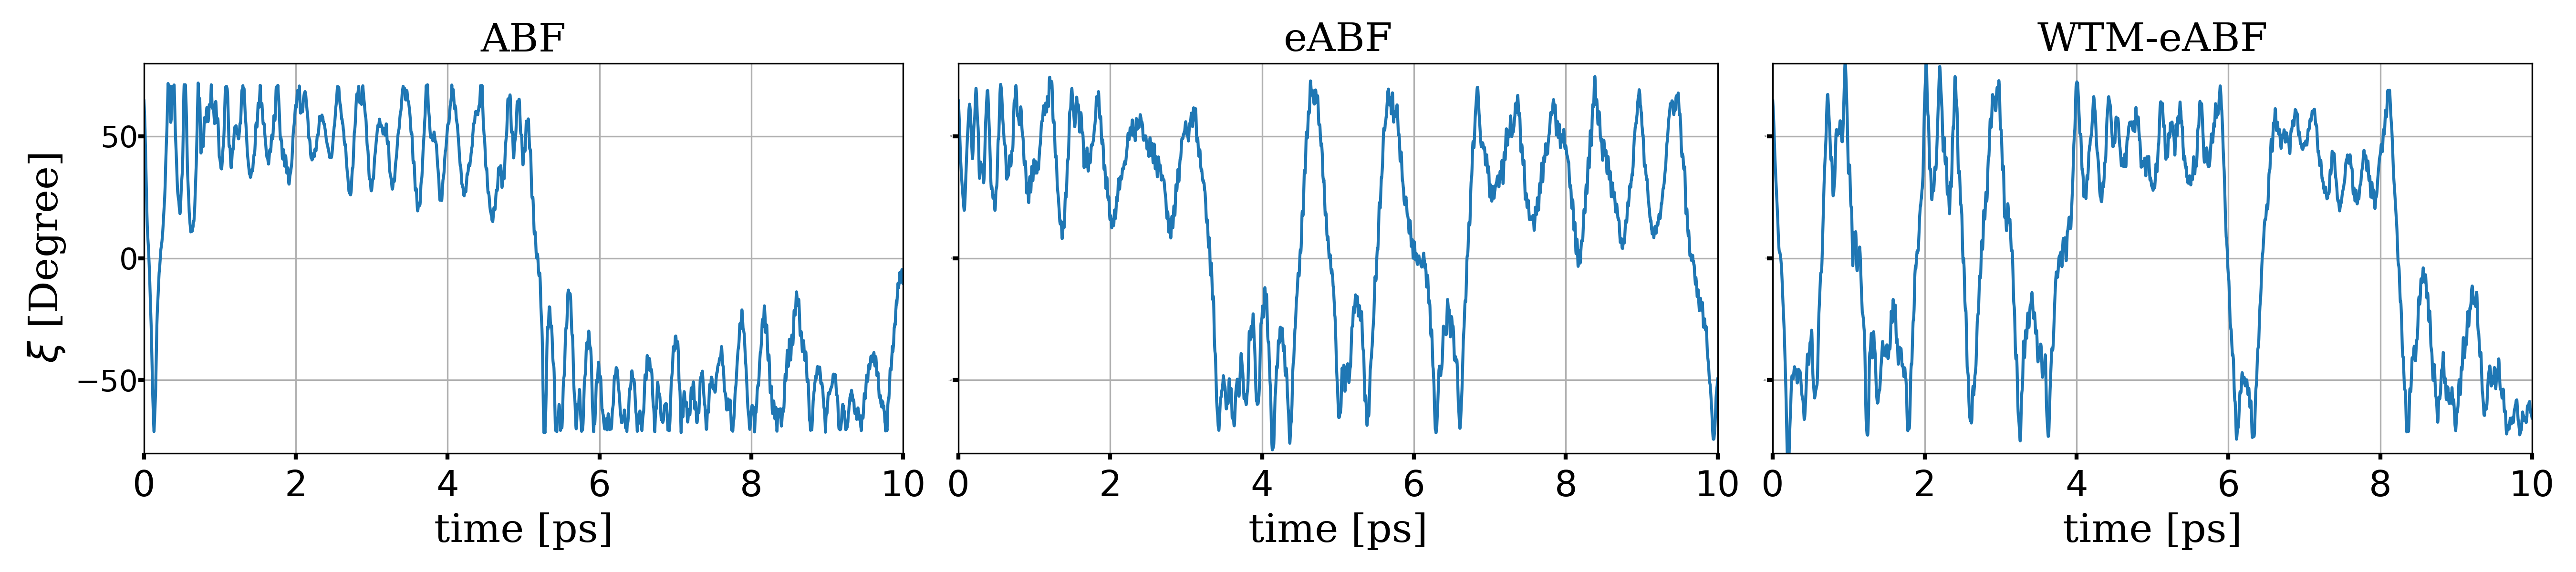
\includegraphics[width=0.99\textwidth]{bilder/benchmark/ABF_trajs}
     \caption{Trajectories during ABF, eABF and WTM-eABF simulation.}
     \label{fig:traj ABF}
\end{figure}

\begin{figure}[H]
  \centering
    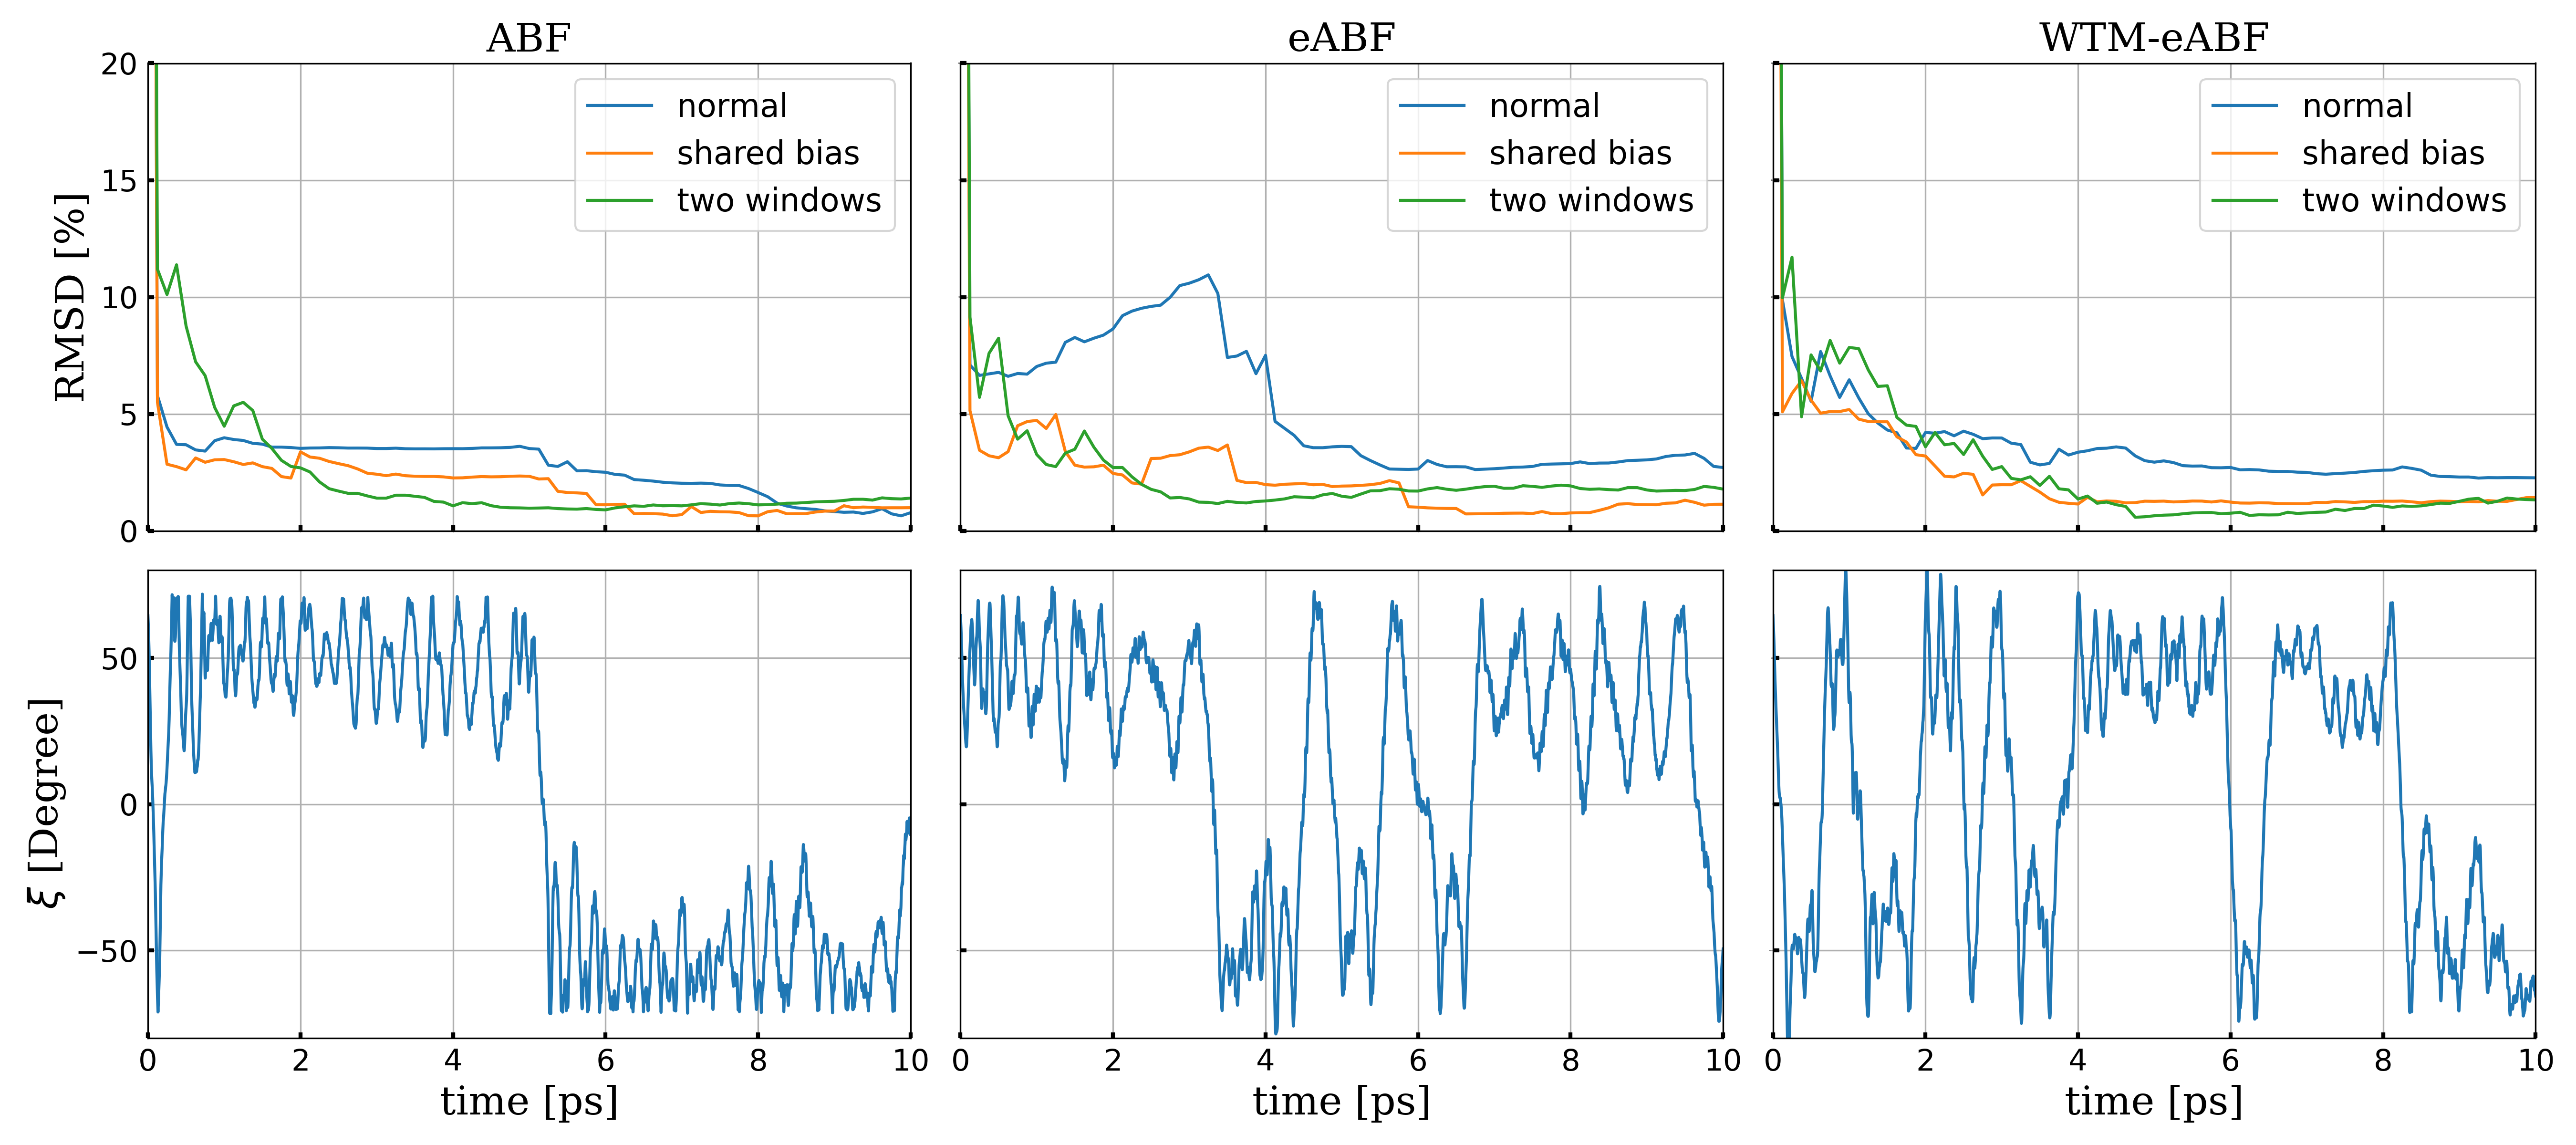
\includegraphics[width=0.99\textwidth]{bilder/benchmark/ABF_acc_benchmark}
   \caption{Convergence of ABF, eABF and WTM-eABF}
   \label{fig:conf ABF}
\end{figure}


% \begin{figure}[H]
%    \centering
%     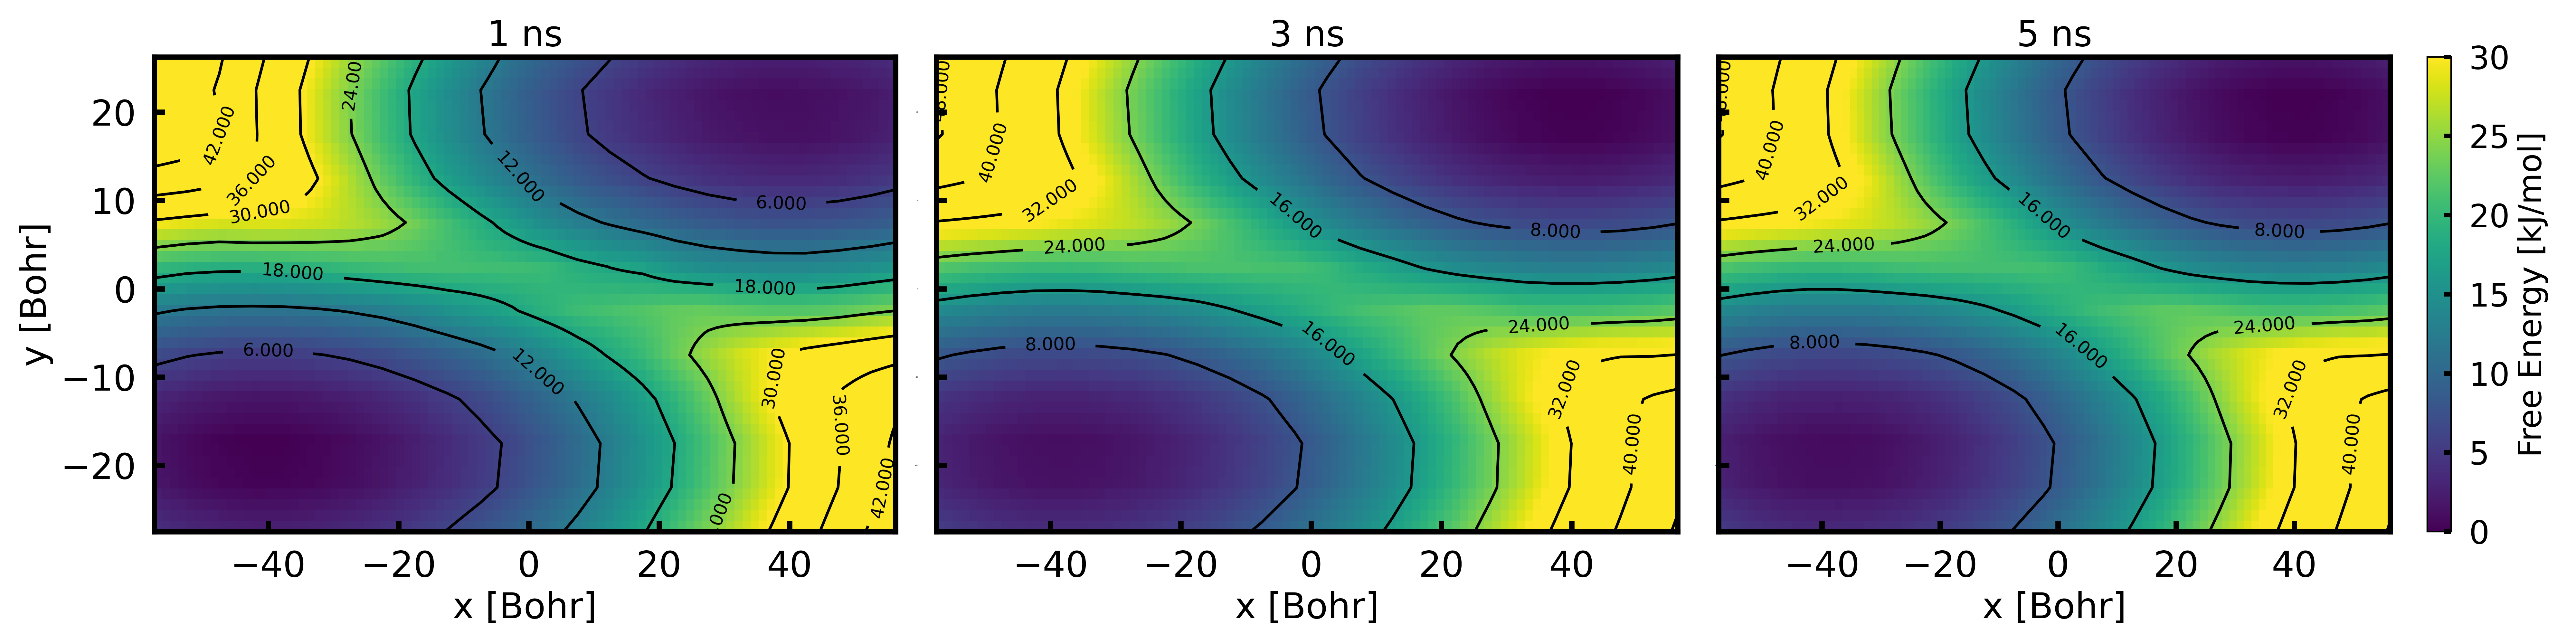
\includegraphics[width=0.99\textwidth]{bilder/test_2D/ABF}  \\
%     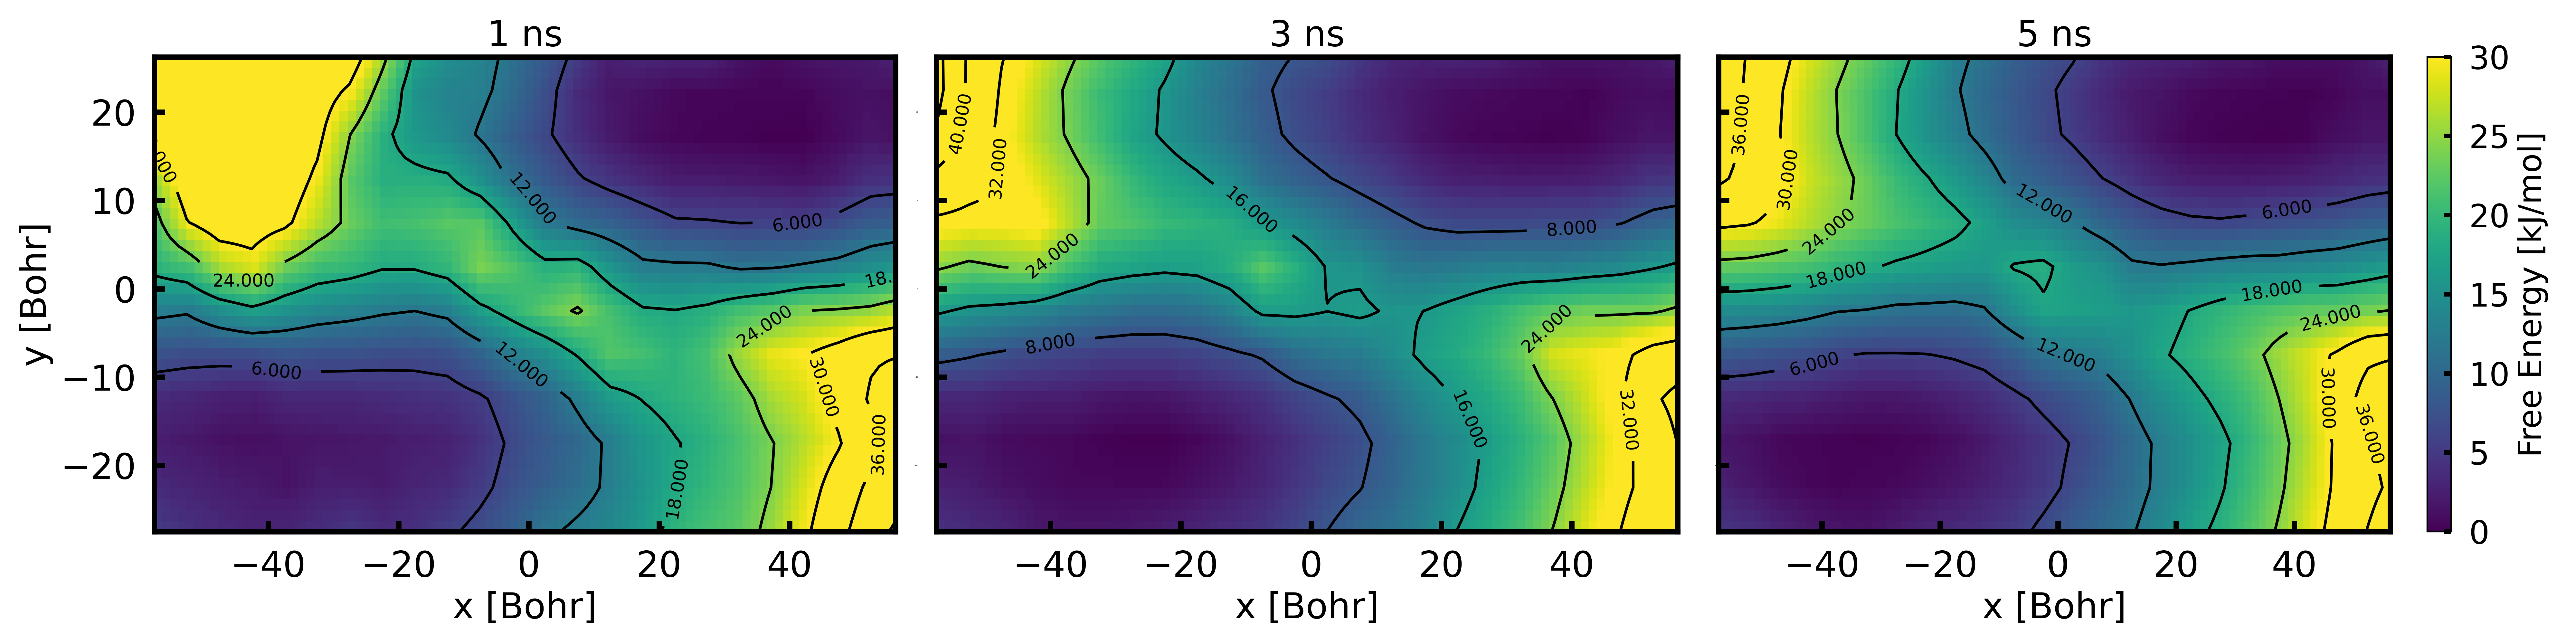
\includegraphics[width=0.99\textwidth]{bilder/test_2D/eABF} \\
%     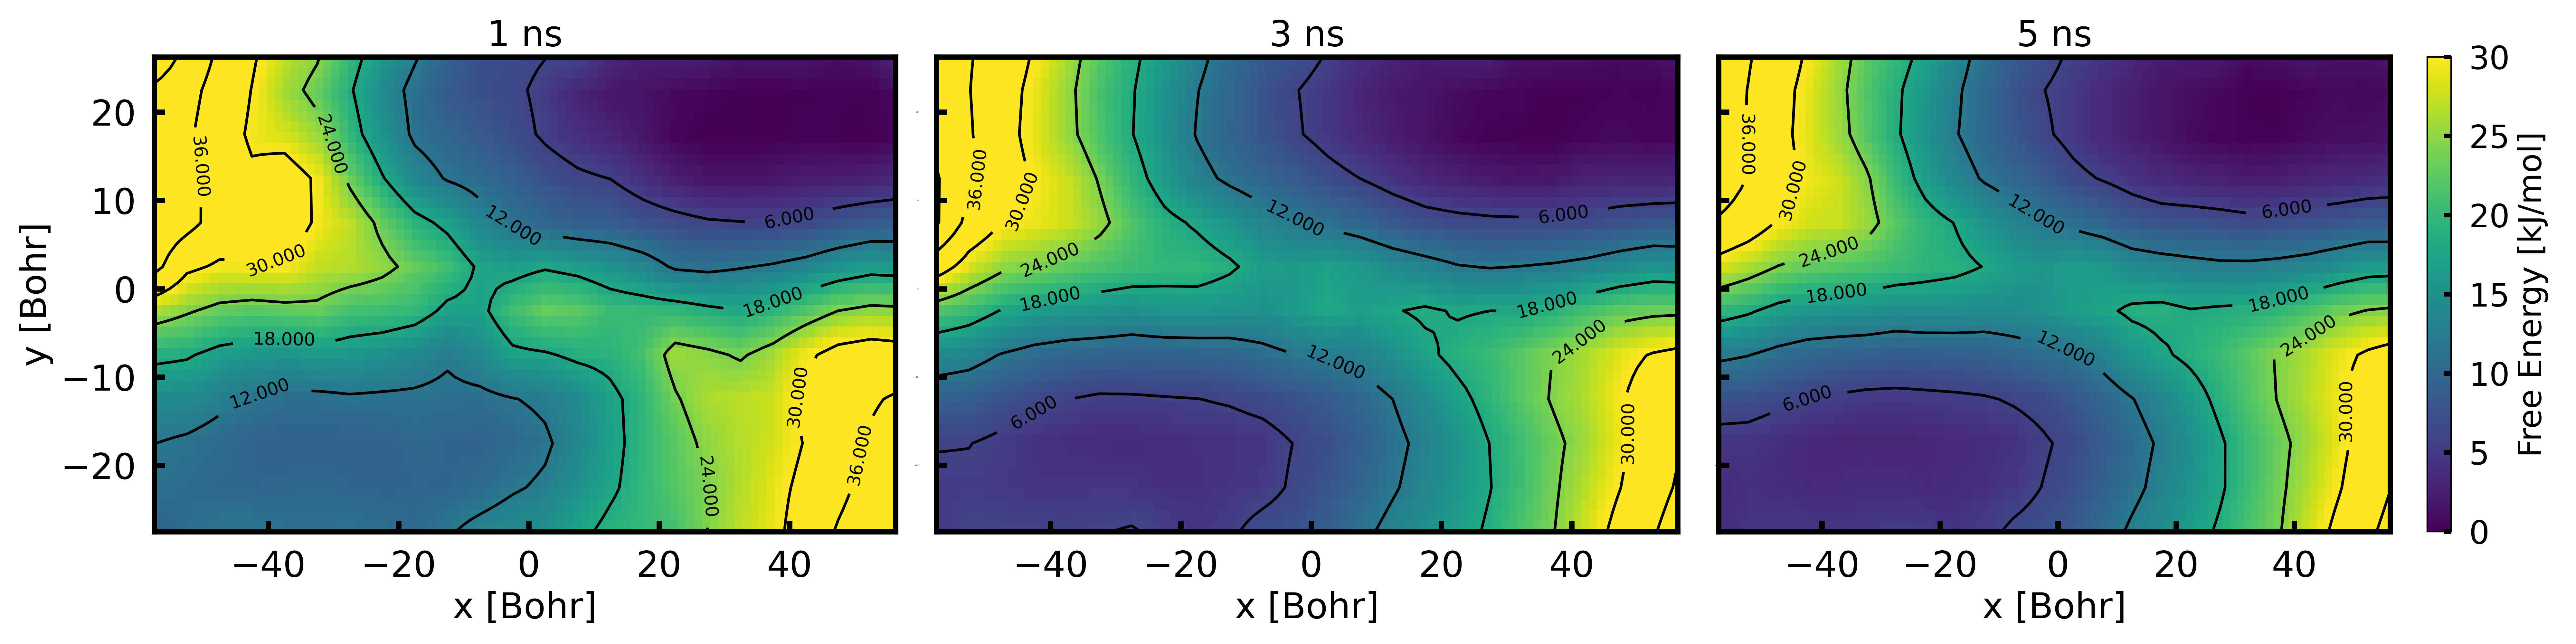
\includegraphics[width=0.99\textwidth]{bilder/test_2D/meta_eABF}
%     \caption{2D ABF, eABF and WTM-eABF test}
% \label{fig:2D ABF}%
% \end{figure}


\section{Application of WTM-eABF to S\textsubscript{n}2-Reactions}
\label{sec:Sn2}


\section{Ring Closing Reaction}
\label{sec:RCR}

\begin{figure}[H]
  \centering
    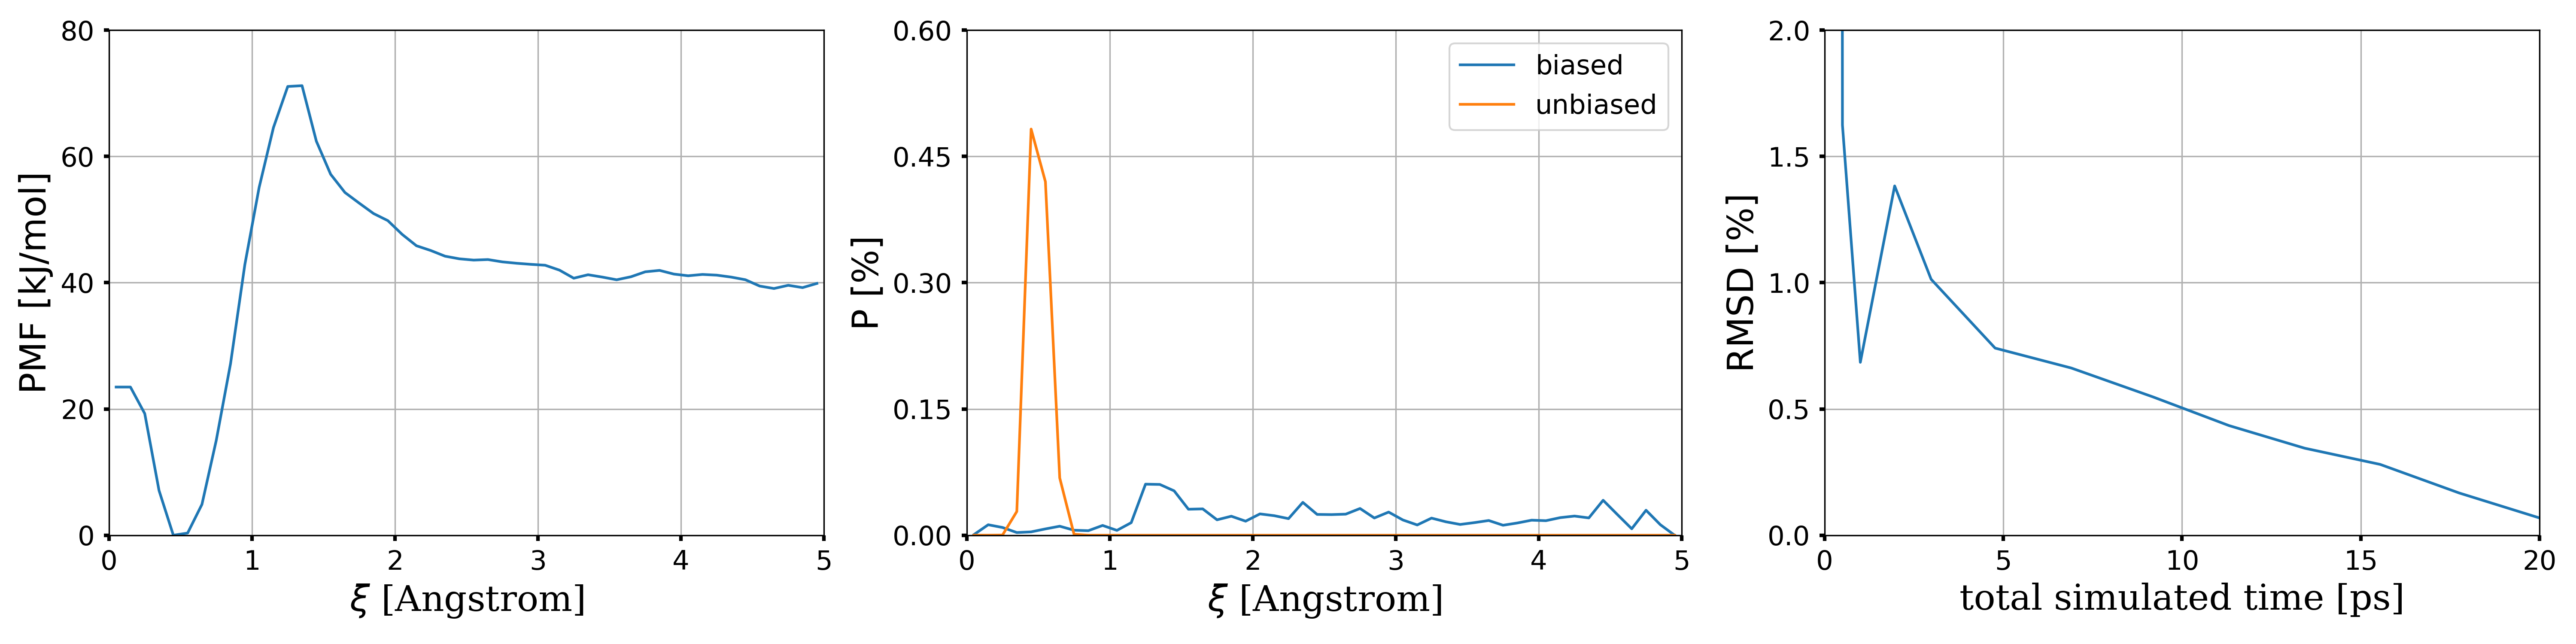
\includegraphics[width=0.99\textwidth]{bilder/results/R2_ool_results}
   \caption{Ring closing reaction}
   \label{fig:ool}
\end{figure}
